\section{Evaluation}
\label{sec:eval}

Following SkyStore~\cite{skystore2025} §6, we answer five questions:
\begin{enumerate}
  \item How much cheaper is ChunkTevict than SkyStore's two-region baselines, object-level SkyStore, and Optimal?
  \item Is the gap storage or transfer, and do chunk hits explain it?
  \item Do the savings hold across SkyStore's three-region workload types and as the number of regions grows?
  \item Do they survive free placement, where no origin copy is pinned?
  \item What does the same replay say about simulated {GET} {RTT} and replay time?
\end{enumerate}
We organize the section as in~\cite{ye2021fast}: datasets, metrics, then results discussed figure by figure.

\subsection{A. Datasets}
\label{sec:eval-data}

To evaluate the method, we use the five complete {IBM} Object Store traces of SkyStore Fig.~5 ({T}15, {T}29, {T}65, {T}78, {T}79)~\cite{snia_ibm2019,skystore2025}.
The traces record timestamp, operation, region, key, and object size, but not payload.
We therefore bind every key to real content once, offline.
A manifest maps each key to a file of matching size class from a pool of versioned public source releases (files extracted from many consecutive Linux kernel versions, plus PostgreSQL and other archives for large objects).
The pooled bytes are chunked with Fast{CDC} (minimum $2$\,KiB, average $8$\,KiB, maximum $64$\,KiB) and fingerprinted with {BLAKE3}; the replay only looks up the resulting chunk ids.
The amount of cross-object sharing is therefore a property of this binding, not of the original {IBM} workload; we return to this point in Section~\ref{sec:eval-threats}.
Two-region runs use SkyStore type~E (base and cache).
Three-, six-, and nine-region runs use types {A}--{D} (uniform, region-aware, aggregation, replication).

{T}15 is write-heavy with many one-hit objects: Always Evict and TevictRanges stay close at object granularity, while Always Store and {AWS} Multi-Region pay a second replica that is rarely reread.

{T}29 is also write-heavy, but objects are tiny and the trace exceeds $12$ million requests.
{GET}s miss often at chunk grain ({GET} hit $43.8\%$ in two regions), yet {PUT}s reuse $97.0\%$ of unique chunks, so object-level clocks still store and move whole keys.

{T}65 is read-heavy and hot.
Almost every {GET} chunk hits locally ($99.8\%$ in two regions), so Always Evict pays transfer on every miss while Always Store and SkyStore stay cheap---and still several times ChunkTevict, because they keep full objects.

{T}78 is read-heavy at high volume ($2.41$ million operations).
Always Evict is catastrophic; $T_{\mathrm{even}}$ and TevictRanges beat Always Store, as in SkyStore §6.3, but remain far above the unique-chunk bill.

{T}79 has large objects and a long {GET} tail.
Always Store and {AWS} Multi-Region keep full replicas for the whole trace; ChunkTevict stores only unique uids.

\subsection{B. Metrics and Setup}
\label{sec:eval-metrics}

We evaluate efficiency with two primary metrics, following~\cite{ye2021fast}: monetary cost without request charges, and overall replay time.
Cost is storage plus transfer at public list prices, matching SkyStore's ``cost without request.''
We report absolute {USD} and the ratio $(\text{policy cost})/(\text{ChunkTevict cost})$.
The same replay records simulated {GET} and {PUT} {RTT} from the directed transfer graph (same-region self-loop $=1$\,ms).
A {GET} miss pays the {RTT} of the chosen edge; ChunkTevict takes the maximum over missing chunks fetched in parallel.
This is a lookup on the price graph, not SkyStore §6.6 end-to-end client latency on a live three-cloud deployment.
{PUT} {RTT} is $1$\,ms for every policy (local write).

Policies follow SkyStore §6.2.2--§6.4.
Two-region Fig.~5 plots Always Evict, Always Store, $T_{\mathrm{even}}$, {TTL}-{CC}, {EWMA}, and {AWS} Multi-Region Bucket; Table~3 separately reports cost versus SkyStore's offline object-level Optimal.
Three-region Table~4 replaces {AWS} Multi-Region with JuiceFS.
Our counterpart figures keep those baselines and change the denominator to ChunkTevict; object-level SkyStore appears as an extra row so the gap versus the original system is explicit.
{TTL} is SkyStore's \texttt{calculate\_ttl}; ChunkTevict only changes the unit from objects to unique chunks.

Two- and three-region results in this section are \textbf{fixed-base ({FB})}, matching SkyStore Fig.~5 and Table~4.
Scale plots follow SkyStore Fig.~6 (type~A cost divided by that policy's own three-region cost) on all five traces, including {T}29 at six and nine regions.
Free placement uses SkyStore Table~5's set (Always Evict, Always Store, JuiceFS, SkyStore, ChunkTevict).
Three-region free placement is complete for five traces; six- and nine-region {T}29 JuiceFS cells are omitted where the 29\,{GB} host ran out of memory.

All experiments run on an 8-v{CPU}, $29$\,{GB} host.
{CDC} is performed once offline; the replay only looks up uids.
Manifest metadata is $40$\,B per chunk reference and is excluded from the dollar bill.

\subsection{C. Numerical Results and Discussion}

\subsubsection{C1. Two-region cost (SkyStore Fig.~5)}
\label{sec:eval-2reg}

SkyStore Fig.~5 is two-region fixed-base type~E: $y=$ baseline cost / SkyStore, $x=$ Always Evict, Always Store, $T_{\mathrm{even}}$, {TTL}-{CC}, {EWMA}, {AWS} Multi-Region.
Tables~\ref{tab:2reg-abs}--\ref{tab:2reg-ratio} use that same $x$ set with $y=$ cost / ChunkTevict.
{AWS} Multi-Region is asynchronous replication on {PUT} to the other region.
{TTL}-{CC} is the stochastic cache {TTL}; {EWMA} uses $\alpha{=}0.5$.
Object-level SkyStore and Optimal play SkyStore Table~3's role and sit in Table~\ref{tab:2reg-opt}.

\begin{table}[t]
\centering
\caption{Two-region {FB} cost (USD without request), SkyStore Fig.~5 policy set.}
\label{tab:2reg-abs}
\setlength{\tabcolsep}{2.4pt}
{\scriptsize
\begin{tabular}{lrrrrrrr}
\toprule
Trace & Evict & Store & Teven & {TTL}-{CC} & {EWMA} & {AWS}-{MR} & ChunkT. \\
\midrule
T15 & 92.79 & 141.78 & 95.95 & 92.40 & 92.79 & 179.33 & 25.22 \\
T29 & 4.60 & 7.15 & 5.02 & 5.57 & 4.60 & 8.48 & 0.39 \\
T65 & 55.06 & 4.39 & 6.32 & 4.86 & 15.91 & 4.41 & 2.01 \\
T78 & 62.91 & 24.02 & 17.81 & 19.21 & 22.90 & 28.96 & 2.50 \\
T79 & 356.37 & 540.17 & 340.83 & 343.25 & 339.72 & 570.71 & 51.92 \\
\bottomrule
\end{tabular}}
\end{table}

\begin{table}[t]
\centering
\caption{Two-region {FB} cost / ChunkTevict (SkyStore Fig.~5 baselines).}
\label{tab:2reg-ratio}
\setlength{\tabcolsep}{2.4pt}
{\scriptsize
\begin{tabular}{lrrrrrrr}
\toprule
Trace & Evict & Store & Teven & {TTL}-{CC} & {EWMA} & {AWS}-{MR} & ChunkT. \\
\midrule
T15 & $3.68\times$ & $5.62\times$ & $3.80\times$ & $3.66\times$ & $3.68\times$ & $7.11\times$ & $1.00\times$ \\
T29 & $11.75\times$ & $18.26\times$ & $12.83\times$ & $14.23\times$ & $11.75\times$ & $21.66\times$ & $1.00\times$ \\
T65 & $27.39\times$ & $2.18\times$ & $3.14\times$ & $2.42\times$ & $7.92\times$ & $2.19\times$ & $1.00\times$ \\
T78 & $25.12\times$ & $9.59\times$ & $7.11\times$ & $7.67\times$ & $9.15\times$ & $11.57\times$ & $1.00\times$ \\
T79 & $6.86\times$ & $10.40\times$ & $6.56\times$ & $6.61\times$ & $6.54\times$ & $11.0\times$ & $1.00\times$ \\
\bottomrule
\end{tabular}}
\end{table}

\begin{table}[t]
\centering
\caption{Two-region {FB} versus object-level SkyStore and Optimal (SkyStore Table~3).}
\label{tab:2reg-opt}
\setlength{\tabcolsep}{3.2pt}
{\scriptsize
\begin{tabular}{lrrr}
\toprule
Trace & SkyStore & Optimal & ChunkT. \\
\midrule
T15 & 92.02 ($3.65\times$) & 90.90 ($3.60\times$) & 25.22 \\
T29 & 4.62 ($11.80\times$) & 4.59 ($11.73\times$) & 0.39 \\
T65 & 4.39 ($2.18\times$) & 4.56 ($2.27\times$) & 2.01 \\
T78 & 16.79 ($6.71\times$) & 16.30 ($6.51\times$) & 2.50 \\
T79 & 337.02 ($6.49\times$) & 323.48 ($6.23\times$) & 51.92 \\
\bottomrule
\end{tabular}}
\end{table}

\begin{figure}[t]
\centering
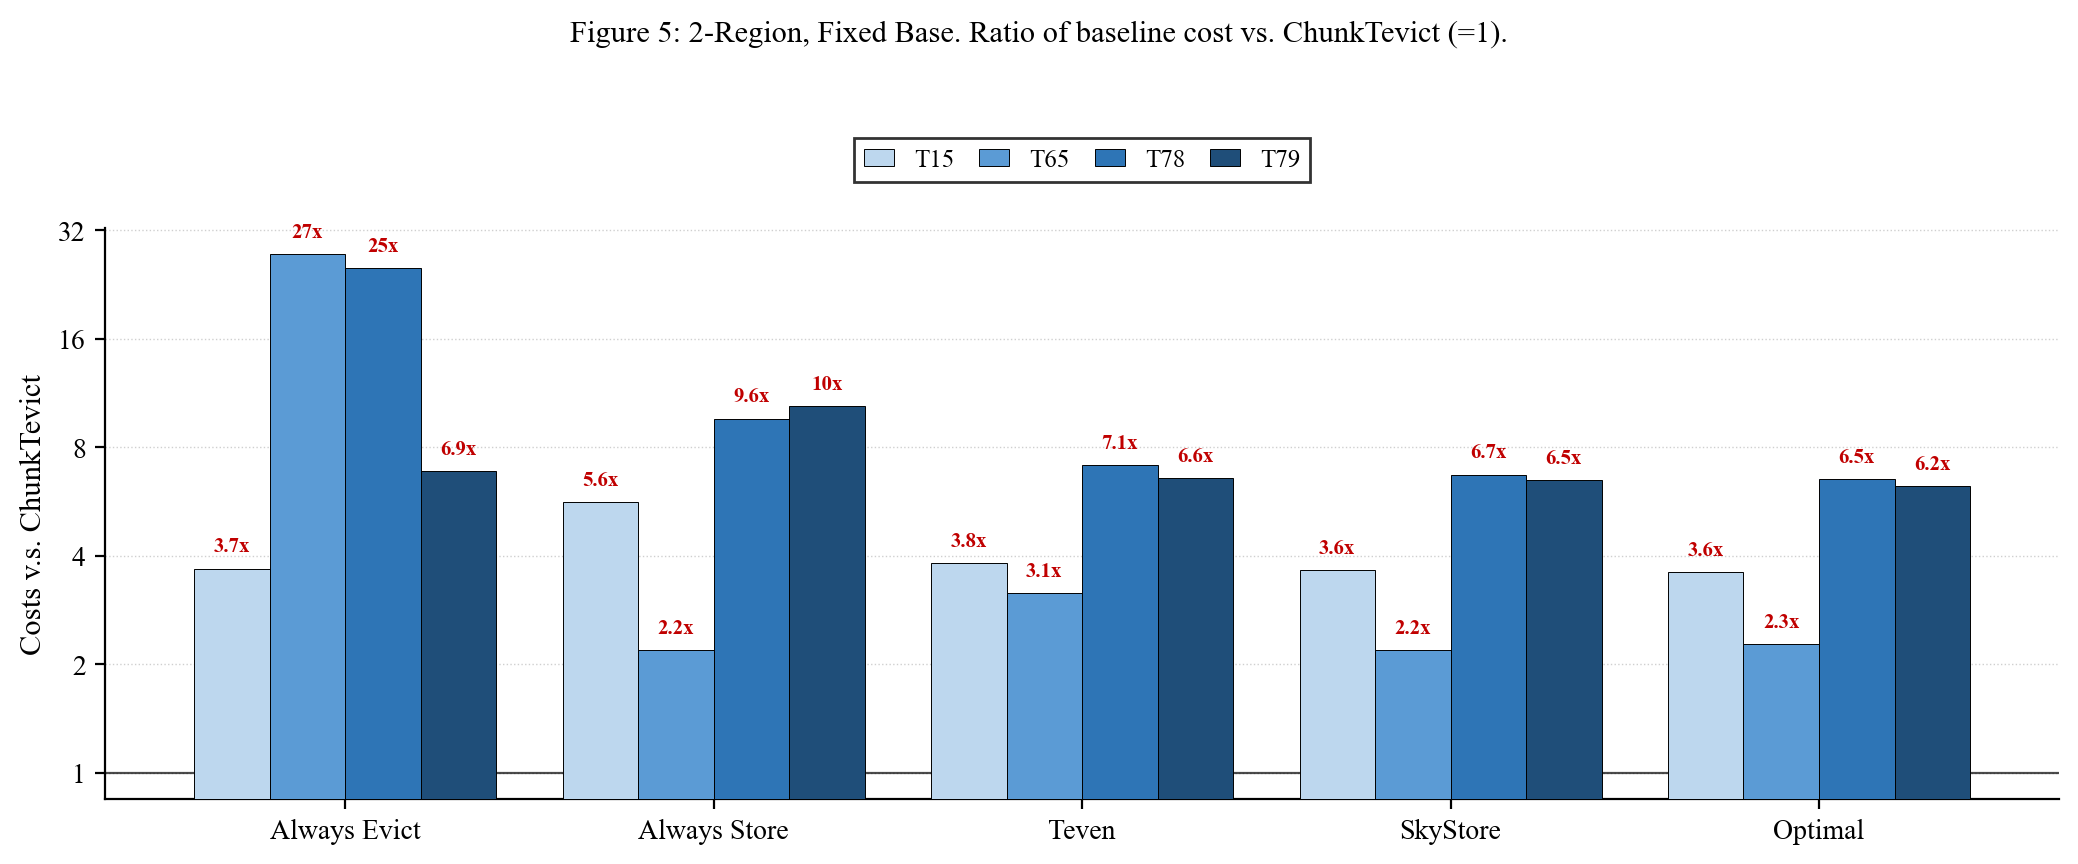
\includegraphics[width=\columnwidth]{figures/fig5_2reg_ratios.png}
\caption{Two-region {FB} cost / ChunkTevict for SkyStore Fig.~5 baselines (Always Evict, Always Store, $T_{\mathrm{even}}$, {TTL}-{CC}, {EWMA}, {AWS} Multi-Region).}
\label{fig:2reg-ratios}
\end{figure}

As shown in Fig.~\ref{fig:2reg-ratios} and Tables~\ref{tab:2reg-abs}--\ref{tab:2reg-opt}, ChunkTevict is cheaper on every trace; the alternatives are low or comparable in specific cases and become much more expensive in others---the same pattern SkyStore §6.3 reports against TevictRanges, now with unique chunks as the denominator.

On {T}15, {TTL}-{CC} tracks object-level SkyStore ($3.66\times$ versus $3.65\times$ ChunkTevict): stochastic cache {TTL}s do not beat TevictRanges by much, and both remain several times ChunkTevict.
Always Store and {AWS} Multi-Region pay a second replica that one-hit writes rarely reread ($5.62\times$ and $7.11\times$).
{EWMA} collapses to Always Evict ($3.68\times$).

{T}29 is the extreme.
Objects are tiny and {GET}s are miss-heavy (ChunkTevict {GET} chunk hit $43.8\%$), so Always Store and {AWS} Multi-Region pay $18$--$22\times$ ChunkTevict while object-level SkyStore is still $11.80\times$.
{EWMA} again matches Always Evict ($11.75\times$).

On {T}65, Always Evict is catastrophic ($27.39\times$) because hot {GET}s miss a remote object every time.
Always Store and {AWS} Multi-Region sit at $2.18\times$ and $2.19\times$: they buy local hits with full-object {GB}$\cdot$h, yet still trail ChunkTevict, whose {GET} chunk hit is $99.8\%$.
{EWMA} only partially closes the gap ($7.92\times$).
$T_{\mathrm{even}}$ and {TTL}-{CC} stay close to SkyStore ($3.14\times$ and $2.42\times$ versus SkyStore $2.18\times$).

On {T}78, Always Evict is again $25.12\times$.
$T_{\mathrm{even}}$ ($7.11\times$) beats Always Store ($9.59\times$), as SkyStore observes when a fixed network-break-even {TTL} is better than never evicting, but TevictRanges at object grain ($6.71\times$) is still far from the unique-chunk bill ($2.50$ {USD}).

On {T}79, Always Store and {AWS} Multi-Region keep large objects for the whole trace ($10.40\times$ and $11.0\times$).
TevictRanges, $T_{\mathrm{even}}$, {TTL}-{CC}, and {EWMA} cluster around $6.5\times$ ChunkTevict.

Object-level Optimal remains $2.27$--$11.73\times$ ChunkTevict (Table~\ref{tab:2reg-opt}).
Future knowledge of \emph{object} accesses does not create a unique-chunk clock: Optimal still stores and moves whole keys.
On {T}65 the artifact's Optimal ($\$4.56$) is slightly above SkyStore ($\$4.39$), so we treat it as a strong object-level reference rather than a strict lower bound.

\subsubsection{C2. Why ChunkTevict saves (storage versus transfer)}
\label{sec:eval-why}

Fig.~\ref{fig:2reg-comp} splits the two-region bill.
Let $\Delta$ be SkyStore minus ChunkTevict.
The storage share of $\Delta$ is $96.7\%$ ({T}15), $95.1\%$ ({T}29), $96.5\%$ ({T}65), $87.8\%$ ({T}78), and $92.6\%$ ({T}79).
Transfer still drops---{T}78 SkyStore transfer is $2.08$ versus ChunkTevict $0.34$ {USD}---but most of the dollar gap is {GB}$\cdot$h that object replicas keep alive.

\begin{figure}[t]
\centering
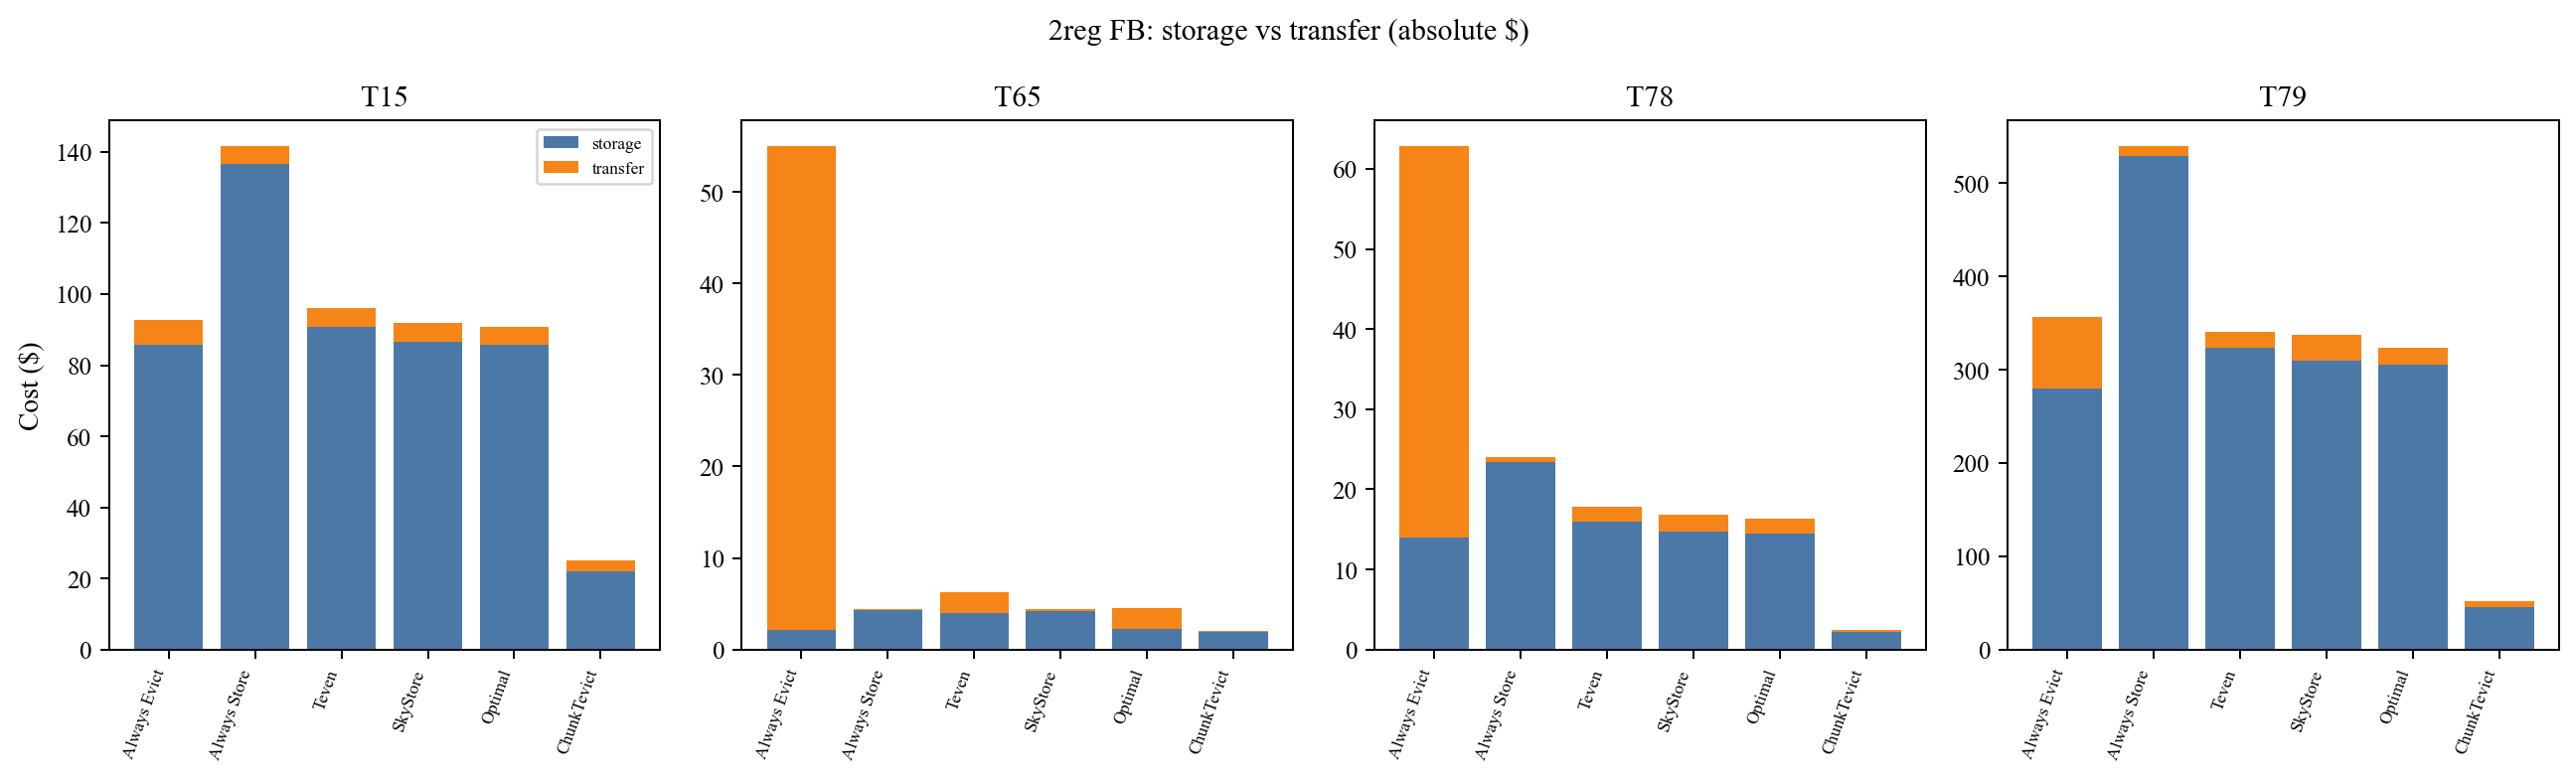
\includegraphics[width=\columnwidth]{figures/fig5_2reg_components.png}
\caption{Two-region {FB} storage versus transfer for SkyStore and ChunkTevict. Storage accounts for $88$--$97\%$ of the gap.}
\label{fig:2reg-comp}
\end{figure}

Table~\ref{tab:hits} reports the fraction of chunk references that find a local uid.
{GET} chunk hits exceed $99\%$ on {T}65/{T}78 in two regions and in every three-region type~A cell we report; two-region {T}15 is harder ({GET} $55.8\%$) and {T}29 is miss-heavy ({GET} $43.8\%$) yet still beats object-level SkyStore by $11.80\times$ because {PUT}s reuse $97.0\%$ of chunks and storage is charged per uid.
Object-level Optimal cannot record those hits: a miss is all-or-nothing on the key.

\begin{table}[t]
\centering
\caption{ChunkTevict local chunk-hit rate (references, not objects).}
\label{tab:hits}
\setlength{\tabcolsep}{3.4pt}
{\scriptsize
\begin{tabular}{llrr}
\toprule
Setup & Trace & {PUT} hit & {GET} hit \\
\midrule
2-reg E & T15 & $82.3\%$ & $55.8\%$ \\
2-reg E & T29 & $97.0\%$ & $43.8\%$ \\
2-reg E & T65 & $39.7\%$ & $99.8\%$ \\
2-reg E & T78 & $87.9\%$ & $99.2\%$ \\
2-reg E & T79 & $81.3\%$ & $88.7\%$ \\
3-reg A & T15 & $70\%$ & $85\%$ \\
3-reg A & T65 & $29\%$ & $99.7\%$ \\
3-reg A & T78 & $81\%$ & $99.5\%$ \\
3-reg A & T79 & $67\%$ & $97.5\%$ \\
\bottomrule
\end{tabular}}
\end{table}

\subsubsection{C3. Simulated {GET} {RTT}}
\label{sec:eval-lat}

Table~\ref{tab:lat} reports two-region {T}65 and {T}78 (hot versus high-volume) from the same replay as C1.
Same-region hits are $1$\,ms; a miss is the paid-edge {RTT} ($68.3$\,ms on this pair); ChunkTevict takes the max over missing chunks fetched in parallel.

On {T}65, ChunkTevict's average {GET} is $1.6$\,ms with p99 $=1$\,ms, against SkyStore $1.7$\,ms / p99 $68.3$\,ms: object misses still pay the full {RTT} even when most chunks would have hit.
Always Evict and {EWMA} stay at the miss {RTT} ($68.3$\,ms and $44.0$\,ms average).
Always Store and {AWS} Multi-Region sit at $1$--$1.5$\,ms because every object is already local---they buy that latency with the storage bill in Table~\ref{tab:2reg-abs}.
{T}78 is noisier: ChunkTevict $6.2$\,ms average matches SkyStore $6.3$\,ms; both still have a $68.3$\,ms p99 from cold unique chunks.

\begin{table}[t]
\centering
\caption{Two-region simulated {GET} {RTT} (ms) from the transfer-graph edge. {PUT} is $1$\,ms for every policy.}
\label{tab:lat}
\setlength{\tabcolsep}{2.8pt}
{\scriptsize
\begin{tabular}{lrrrrrr}
\toprule
 & \multicolumn{3}{c}{{GET} {T}65} & \multicolumn{3}{c}{{GET} {T}78} \\
\cmidrule(lr){2-4} \cmidrule(lr){5-7}
Policy & avg & p90 & p99 & avg & p90 & p99 \\
\midrule
Always Evict & 68.3 & 68.3 & 68.3 & 68.3 & 68.3 & 68.3 \\
Always Store & 1.5 & 1.0 & 1.0 & 2.7 & 1.0 & 68.3 \\
$T_{\mathrm{even}}$ & 9.5 & 68.3 & 68.3 & 5.8 & 1.0 & 68.3 \\
{TTL}-{CC} & 3.7 & 1.0 & 68.3 & 5.5 & 1.0 & 68.3 \\
{EWMA} & 44.0 & 68.3 & 68.3 & 24.6 & 68.3 & 68.3 \\
{AWS}-{MR} & 1.0 & 1.0 & 1.0 & 1.0 & 1.0 & 1.0 \\
SkyStore & 1.7 & 1.0 & 68.3 & 6.3 & 1.0 & 68.3 \\
ChunkTevict & 1.6 & 1.0 & 1.0 & 6.2 & 1.0 & 68.3 \\
\bottomrule
\end{tabular}}
\end{table}

\subsubsection{C4. Three-region workload types (SkyStore Table~4)}
\label{sec:eval-3reg}

SkyStore Table~4 reports, for each policy, the mean over traces of $(\text{policy cost})/(\text{SkyStore cost})$, with rows Always Evict, Always Store, $T_{\mathrm{even}}$, {TTL}-{CC}, {EWMA}, and JuiceFS.
We keep that row set and the type {A}--{D} columns, change the denominator to ChunkTevict, and add a SkyStore row (Table~\ref{tab:3reg-t4}, Fig.~\ref{fig:3reg-t4}).

\begin{table}[t]
\centering
\caption{Three-region {FB}: mean over five traces of cost / ChunkTevict, SkyStore Table~4 workload types.}
\label{tab:3reg-t4}
\setlength{\tabcolsep}{2.8pt}
{\scriptsize
\begin{tabular}{lrrrrr}
\toprule
Policy & A unif. & B region & C agg. & D repl. & Mean \\
\midrule
Always Evict & $23.67\times$ & $42.00\times$ & $34.20\times$ & $25.60\times$ & $31.37\times$ \\
Always Store & $8.38\times$ & $7.14\times$ & $7.41\times$ & $8.43\times$ & $7.84\times$ \\
$T_{\mathrm{even}}$ & $7.19\times$ & $6.66\times$ & $6.82\times$ & $7.23\times$ & $6.98\times$ \\
{TTL}-{CC} & $7.60\times$ & $6.49\times$ & $6.78\times$ & $7.71\times$ & $7.15\times$ \\
{EWMA} & $10.15\times$ & $10.81\times$ & $10.16\times$ & $10.35\times$ & $10.37\times$ \\
JuiceFS & $14.29\times$ & $15.42\times$ & $15.63\times$ & $14.31\times$ & $14.91\times$ \\
SkyStore & $6.43\times$ & $6.29\times$ & $6.43\times$ & $6.45\times$ & $6.40\times$ \\
ChunkTevict & $1.00\times$ & $1.00\times$ & $1.00\times$ & $1.00\times$ & $1.00\times$ \\
\bottomrule
\end{tabular}}
\end{table}

\begin{figure}[t]
\centering
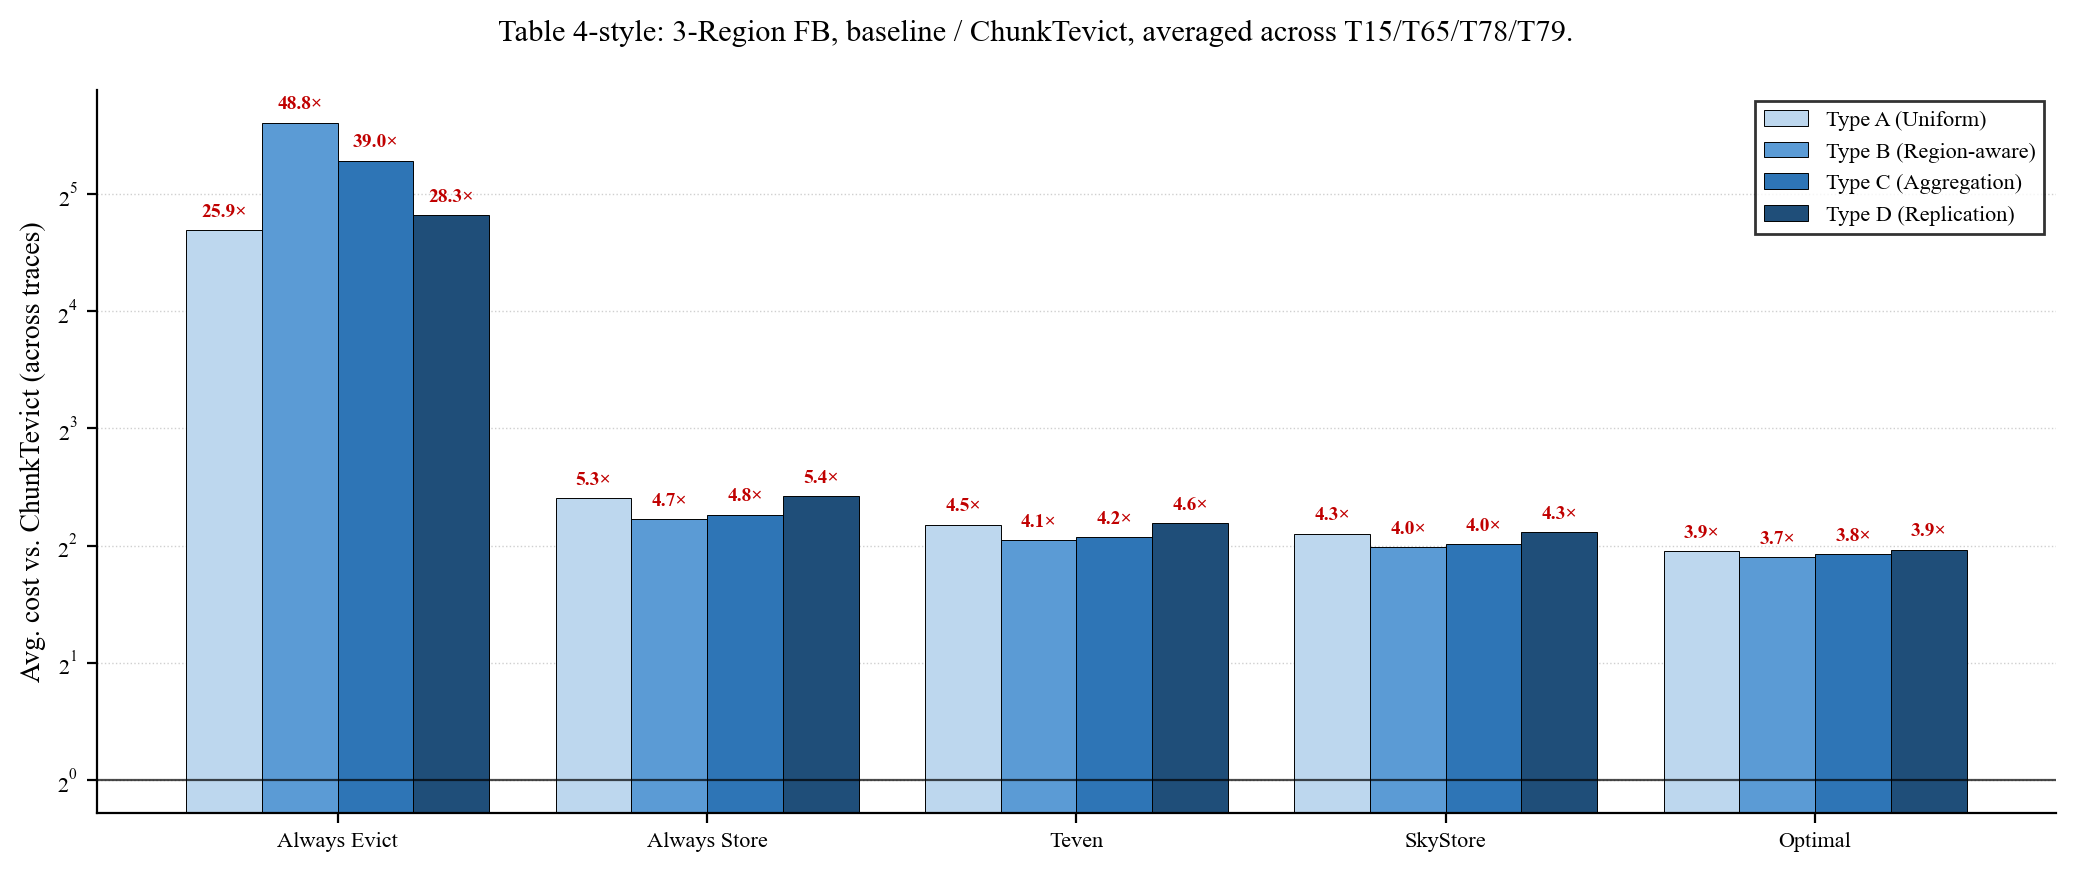
\includegraphics[width=\columnwidth]{figures/fig5_3reg_table4.png}
\caption{Three-region {FB} mean cost / ChunkTevict by SkyStore Table~4 workload type (five traces).}
\label{fig:3reg-t4}
\end{figure}

Averaged over the five traces, SkyStore is $6.40\times$ ChunkTevict (type~B $6.29\times$, type~A $6.43\times$).
{T}29 dominates the mean: ChunkTevict is $\$0.36$ on three-region {T}29 while SkyStore remains $\$5.3$--$5.7$, so that one trace is about $15\times$ by itself.
JuiceFS is $14.91\times$ on average---SkyStore Table~4 already reported JuiceFS $1.9$--$4.8\times$ SkyStore; we see the same industrial baseline after changing the denominator.
{TTL}-{CC} tracks SkyStore ($7.15\times$ versus $6.40\times$).
{EWMA} sits between Always Evict and $T_{\mathrm{even}}$ ($10.37\times$).
Type~B (region-aware) inflates Always Evict the most ($42.00\times$) because misses concentrate on expensive edges, while ChunkTevict hits unique chunks locally.
Type~A (uniform) is the mildest Evict penalty ($23.67\times$).

\subsubsection{C5. Scaling the number of regions (SkyStore Fig.~6)}
\label{sec:eval-scale}

Table~\ref{tab:scale} reports type~A cost divided by \emph{that policy's own} three-region cost, matching SkyStore Fig.~6.
Over five traces, SkyStore's mean 6-region / 3-region ratio is $1.25$ and 9-region / 3-region is $1.52$; ChunkTevict is $1.53$ and $2.06$.
{T}15, {T}29, and {T}79 stay relatively flat for SkyStore ($1.03$--$1.28$), as in the original Fig.~6; object-level {T}29 barely grows ($\$5.35\rightarrow\$5.50\rightarrow\$5.67$) because write-heavy keys already pay an immortal origin.
ChunkTevict on {T}29 grows $1.72\times$ / $2.39\times$ because unique chunks become resident in more caches---the same mechanism that saves dollars in two and three regions.
{T}65 still grows fastest for both systems (ChunkTevict $2.84\times$ at nine regions) as uniform {GET}s spread.
JuiceFS type~A is $2.05\times$ and $3.17\times$ its own three-region bill at six and nine regions ({T}15 $312.87\rightarrow 640.97\rightarrow 990.36$), matching SkyStore Table~5's warning that replicate-on-write storage scales with region count.
Nine-region JuiceFS {T}29 is missing (out-of-memory on the evaluation host).

\subsubsection{C6. Free placement (SkyStore Table~5)}
\label{sec:eval-fp}

SkyStore Table~5 evaluates free placement ({FP}), where no region holds an immortal origin copy.
We use its policy set---Always Evict, Always Store, JuiceFS---and add SkyStore and ChunkTevict (Table~\ref{tab:fp3}).
Averaged over five traces and four types, SkyStore is $5.00\times$ ChunkTevict, lower than the {FB} mean of $6.40\times$.
The drop is consistent with SkyStore §6.5: without a pinned base, object-level TevictRanges already evicts more aggressively.
The remaining gap is chunk billing.

Type~C is the outlier ($6.55\times$), driven by {T}29: ChunkTevict costs $\$0.34$ there against SkyStore's $\$4.87$.
On the other {T}29 types, ChunkTevict under {FP} is \emph{more} expensive than under {FB} (type~A: $\$1.24$ versus $\$0.36$; type~B: $\$0.91$).
Without a pinned origin, chunks shared by many small objects expire and must be fetched back from a remaining holder, so for write-heavy traces with heavy reuse the pinned origin is worth more to ChunkTevict than to SkyStore.
Six- and nine-region {FP} JuiceFS {T}29 cells exceeded the host's memory and are omitted.

\begin{table}[t]
\centering
\caption{Three-region {FP}: mean over five traces of cost / ChunkTevict (SkyStore Table~5 policy set).}
\label{tab:fp3}
\setlength{\tabcolsep}{2.8pt}
{\scriptsize
\begin{tabular}{lrrrrr}
\toprule
Policy & A unif. & B region & C agg. & D repl. & Mean \\
\midrule
Always Evict & $21.39\times$ & $50.18\times$ & $44.45\times$ & $23.21\times$ & $34.81\times$ \\
Always Store & $5.70\times$ & $6.03\times$ & $8.71\times$ & $5.75\times$ & $6.55\times$ \\
JuiceFS & $9.52\times$ & $12.94\times$ & $18.34\times$ & $9.53\times$ & $12.58\times$ \\
SkyStore & $4.52\times$ & $4.41\times$ & $6.55\times$ & $4.53\times$ & $5.00\times$ \\
ChunkTevict & $1.00\times$ & $1.00\times$ & $1.00\times$ & $1.00\times$ & $1.00\times$ \\
\bottomrule
\end{tabular}}
\end{table}

\begin{table}[t]
\centering
\caption{Type~A {FB} cost / own 3-region cost (SkyStore Fig.~6). Five traces.}
\label{tab:scale}
\setlength{\tabcolsep}{3.0pt}
{\scriptsize
\begin{tabular}{llrrrr}
\toprule
Policy & Trace & 3-reg \$ & 6/3 & 9/3 \\
\midrule
SkyStore & T15 & 100.05 & $1.03\times$ & $1.06\times$ \\
 & T29 & 5.35 & $1.03\times$ & $1.06\times$ \\
 & T65 & 6.85 & $1.87\times$ & $2.73\times$ \\
 & T78 & 27.84 & $1.21\times$ & $1.45\times$ \\
 & T79 & 398.18 & $1.10\times$ & $1.28\times$ \\
 & mean & --- & $1.25\times$ & $1.52\times$ \\
\midrule
ChunkTevict & T15 & 36.69 & $1.26\times$ & $1.45\times$ \\
 & T29 & 0.36 & $1.72\times$ & $2.39\times$ \\
 & T65 & 3.06 & $1.89\times$ & $2.84\times$ \\
 & T78 & 4.22 & $1.38\times$ & $1.77\times$ \\
 & T79 & 71.18 & $1.39\times$ & $1.84\times$ \\
 & mean & --- & $1.53\times$ & $2.06\times$ \\
\bottomrule
\end{tabular}}
\end{table}

\subsubsection{C7. Overall time}
\label{sec:eval-perf}

Table~\ref{tab:wall} lists wall-clock replay time and operations per second on the 8-v{CPU} host---the counterpart of overall time in~\cite{ye2021fast}, not client {GET}/{PUT} latency.
The heavy traces are {T}78 ($2.41$ million operations, $3.1$\,h in two regions) and {T}29 ($13.0$ million operations, $12.9$\,h in two regions).
{T}79 is only $114$ thousand operations but $41$ ops/s in two regions because objects are large (many uids per request).
Three-region {T}29 is much faster per operation than two-region ($3670$ versus $280$ ops/s) because unique chunks stay hot across three caches.
{CDC} is offline and is not on the replay critical path.
The unique-chunk indexes used by the replay contain $8.63$\,M, $0.13$\,M, $0.25$\,M, $0.67$\,M, and $8.69$\,M uids for {T}15/{T}29/{T}65/{T}78/{T}79; each chunk reference occupies $40$\,B in the manifest and is not added to the storage bill.

\begin{table}[t]
\centering
\caption{ChunkTevict replay wall time on the 8-v{CPU} host.}
\label{tab:wall}
\setlength{\tabcolsep}{3.2pt}
{\scriptsize
\begin{tabular}{llrrrr}
\toprule
Setup & Trace & Ops & Wall (s) & Ops/s & Cost \\
\midrule
2-reg E & T15 & 1\,575\,627 & 5764 & 273 & 25.22 \\
2-reg E & T29 & 13\,019\,220 & 46457 & 280 & 0.39 \\
2-reg E & T65 & 283\,086 & 2517 & 112 & 2.01 \\
2-reg E & T78 & 2\,409\,805 & 11250 & 214 & 2.50 \\
2-reg E & T79 & 114\,227 & 2814 & 41 & 51.92 \\
3-reg A & T15 & 1\,575\,627 & 2575 & 612 & 36.69 \\
3-reg A & T29 & 13\,019\,220 & 3547 & 3670 & 0.36 \\
3-reg A & T65 & 283\,086 & 1486 & 191 & 3.06 \\
3-reg A & T78 & 2\,409\,805 & 8528 & 283 & 4.22 \\
3-reg A & T79 & 114\,227 & 760 & 150 & 71.18 \\
\bottomrule
\end{tabular}}
\end{table}

\subsection{D. Threats to Validity}
\label{sec:eval-threats}

\textbf{Content binding.}
The {IBM} traces carry no payload, so the cross-object sharing that ChunkTevict exploits comes from our binding to versioned public data.
Workloads with little shared content (encrypted, compressed, or unique media objects) would reduce ChunkTevict to object-level SkyStore plus chunk metadata; the absolute ratios should be read as conditional on content that repeats.

\textbf{Two changes at once.}
ChunkTevict both stores each chunk once per region and gives each chunk its own lease.
Our baselines bill whole objects, so the reported ratios include both effects; Section~\ref{sec:eval-why} shows that most of the gap is storage.

\textbf{Request charges and metadata.}
As in SkyStore, cost excludes per-request charges.
A chunk-level store issues more {GET}/{PUT} calls unless chunks are packed into containers, and the chunk index itself occupies $40$\,B per reference.
Latency is a lookup on the transfer graph, not a live multi-cloud measurement.
